% Primarily this section should be about scientific methods and theories you need to evaluate/compare/invent to solve your problems from 1.3.
% In some cases it may be ok to describe different technologies, but the purpose is to describe something and then draw a conclusion from that.
% Example, if you decide to discuss different databases, it may be for the purpose of selecting the best type for your implementation later on (based on for example data representation, scalability, speed, etc.).
% Optimally the problems in 1.3 are not solved by anyone else yet, in which case this section needs to describe how to solve them (new algorithms, mathematical approaches, etc.).
 
% This section can have a lot of subsections (3.1, 3.2, 3.3, etc).

% TODO: Explain Evaluation of values

TODO

\begin{figure}[h]
    \centering
    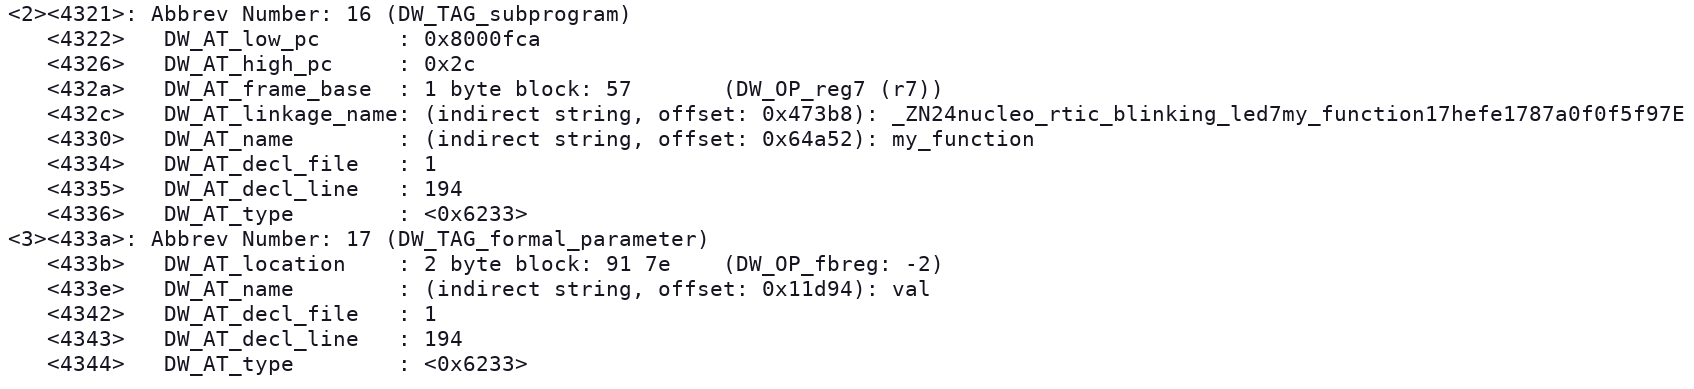
\includegraphics[width=1.0\textwidth]{subprogram-example.png}
    \label{fig:subprogramexample}
\end{figure}

